\graphicspath{{part_0/figures}{part_0/figures/}}


\newcommand{\Rset}{\mathbb{R}}
\newcommand{\IRset}{\mathbb{IR}}



\section{Switched systems}
\label{sec:intro_detailed}

We are interested in continuous-time switched systems subject
to disturbances, described by the set of nonlinear 
ordinary differential equation:
\begin{equation}
  \dot x = f_j(x,d),
  \label{eq:switched_system0}
\end{equation}
 where $x \in \R^n$ is the state
of the system, $j \in U$ is the mode of the system, and $d \in \R^m$ is a bounded
perturbation. The finite set $U = \{ 1, \dots , N \}$ is the set of
switching modes of the system.
The functions $f_j:\R^n \times \R^m \longrightarrow \R^n$, with $j\in U$, are the vector fields
describing the dynamics of each mode $j$ of the system. The system 
can be in only one mode at a time.
We focus on sampled switched systems:
given a sampling period $\tau >0$, switchings will occur
periodically at times $\tau$, $2\tau$, \dots{}
A~switching rule $\sigma(\cdot) : \R^+ \longrightarrow U$
associates to each time $t>0$ the active mode $j \in U$.
A switched system is thus a dynamical system
with piecewise dynamics, and the switching rule selects which mode is active.
Given a switching rule $\sigma(\cdot) : \R^+ \longrightarrow U$, 
and a perturbation $w(\cdot): \R^+ \longrightarrow \R^m$,
we will denote by $\phi(t;t_0,x_0,\sigma,w)$ the state
reached by the system at time $t>t_0$, from the initial 
state $x_0 \in \R^n$ at time $t_0 \geq 0$,
and under control input and perturbation $\sigma$ and $w$ respectively.
% We will call a ``control pattern'' of length $N \in \N$ (pattern for short) a finite sequence of 
% switched modes $\pi = (j_1, j_2, \dots j_N) \in U^N$.



Often, we will consider $\phi(t;t_0,x^0,\sigma,w)$ on the interval 
$0\leq t<\tau$ for which $\sigma(t)$ is equal to a constant, 
say $j\in U$. In this case, we will abbreviate $\phi(t;t_0,x^0,\sigma,w)$ 
as $\phi_j(t;t_0,x^0,w)$. We will also consider $\phi(t;t_0,x^0,\sigma,w)$ 
on the interval $0\leq t<k\tau$
where $k$ is a positive integer, and 
$\sigma(t)$ is equal to a constant, say $j_{k'}$,
on each interval
$[(k'-1)\tau,k'\tau)$ with $1\leq k'\leq k$; in this case,
we will abbreviate $\phi(t;t_0,x^0,\sigma,w)$ as $\phi_\pi(t;t_0,x^0,w)$,
where $\pi$ is a sequence of $k$ modes, also denoted as a control pattern (pattern for short),
of the form $\pi=j_1\cdot j_2\cdot\dots\cdot j_k$. 

We will assume that $\phi(\cdot;t_0,x_0,\sigma,w)$ is {\em continuous} 
at time $k\tau$ for all positive integer $k$.
This means that there is no ``reset'' at time $k'\tau$ ($1\leq k'\leq k$);
the value of 
$\phi_\sigma(t;t_0,x^0,w)$ for $t\in[(k'-1)\tau,k\tau]$
corresponds to the solution of $\dot{x}(u)=f_{j_{k'}}(x(u),w(u))$  for $u\in [0,\tau]$
with initial value $\phi_\sigma((k'-1)\tau;t_0,x^0,w((k'-1)\tau)$.

Given a ``recurrence set'' $R\subset\mathbb{R}^n$ and a ``safety set'' 
$S\subset\mathbb{R}^n$ which contains $R$ ($R\subseteq S$), we are interested in 
the synthesis of a control such that:
starting from any initial point $x\in R$, the controlled trajectory always 
returns to $R$ within a bounded time while never leaving $S$. We suppose that 
sets $R$ and $S$ are compact. Furthermore, we suppose that $S$ is convex.

This is formalized as follows:
\begin{problem}[$(R,S)$-Stability problem]
 Given a switched system of 
 the form \eqref{eq:switched_system0}, a recurrence set $R \subset \R^n$ 
 and a safety set $S \subset \R^n$,
 find a control rule $\sigma : \R^+ \longrightarrow U$ such that, for any initial 
 condition $x_0 \in R$ and any perturbation $w : \R^+ \longrightarrow U$, the following holds:
 \begin{itemize}
  \item Recurrence in $R$: there exists a monotonically strictly 
  increasing sequence of (positive) integers $\{ k_l \}_{l \in \N}$ 
  such that for all $l \in \N$, $\phi(k_l\tau ;t_0,x^0,\sigma,w) \in R$
  \item Stability in $S$: for all $t \in \R^+, \phi(t ;t_0,x^0,\sigma,w) \in S$
 \end{itemize}
\label{prob:RS-stability}
\end{problem}

We also define a similar problem for reachability from a set $R_1 \subset \R^n$
to a set $R_2 \subset \R^n$, where both $R_1$ and $R_2$ are subsets of $S \seq \R^n$.
\begin{problem}[$(R_1,R_2,S)$-Reachability problem]
 Given a switched system of 
 the form \eqref{eq:switched_system0}, two sets $R_1 \subset \R^n$,
 and $R_2 \subset \R^n$,
 and a safety set $S \subset \R^n$,
 find a control rule $\sigma : \R^+ \longrightarrow U$ such that, for any initial 
 condition $x_0 \in R_1$ and any perturbation $w : \R^+ \longrightarrow U$, the following holds:
 \begin{itemize}
  \item Reachability from $R_1$ to $R_2$: there exists an integer $k \in \N_{>0}$ 
  such that $\phi(k\tau ;t_0,x^0,\sigma,w) \in R_2$
  \item Stability in $S$: for all $t \in \R^+, \phi(t ;t_0,x^0,\sigma,w) \in S$
 \end{itemize}
\label{prob:RRS-reachability}
\end{problem}

Another interesting problem is the avoid problem, where one
has to ensure $(R,S)$-stability while avoiding an obstacle, given as a set $B$.
\begin{problem}[$(R,B,S)$-Avoid problem]
  Given a switched system of 
 the form \eqref{eq:switched_system0}, and given three sets $R \subset \R^n$, $S \subset \R^n$, and
  $B \subset \R^n$, with $R \cup B \subset S$ and $R \cap B = \emptyset$, find a
  rule $\sigma : \R^+ \longrightarrow U$ such that, 
  for any initial 
 condition $x_0 \in R$ and any perturbation $w : \R^+ \longrightarrow U$, the following holds:
 \begin{itemize}
  \item Recurrence in $R$: there exists a monotonically strictly 
  increasing sequence of (positive) integers $\{ k_l \}_{l \in \N}$ 
  such that for all $l \in \N$, $\phi(k_l\tau ;t_0,x^0,\sigma,w) \in R$
  \item Stability in $S$: for all $t \in \R^+, \phi(t ;t_0,x^0,\sigma,w) \in S$
 \item Avoid $B$: for all  $t \in \R^+, \phi(t ;t_0,x^0,\sigma,w) \notin B$.
 \end{itemize}
 \label{prob:nl_control}
\end{problem}

In the rest of this chapter, we focus on solving Problem \ref{prob:RS-stability}
of synthesizing controllers for $(R,S)$-stability 
for systems of the form \eqref{eq:switched_system0}, and we will omit 
the disturbance $w$. We thus consider that system \ref{eq:switched_system0}
is fully deterministic. Note that solving Problem~\ref{prob:RRS-reachability} can
be done in a very similar manner (see Section ???).
As a matter of fact, we will not look for {\em time dependent} switching rules $\sigma: \R^+ \lra U$, 
which would require computing infinite sequences of modes, but rather 
look for {\em state-dependent} switching rules, i.e., which depend on 
the state $x$ of the system. This can be performed {\em offline}.
{\todo d\'efinition formelle loi de controle???}


% \subsection{Switched systems}
% \label{sec:switched}
% Let us consider nonlinear switched systems such that
% \begin{equation}
%   \dot x(t) = f_{\sigma (t)}(x(t),d(t))
%   \label{eq:sys}
% \end{equation}
% defined for all $t \geq 0$, where $x(t) \in \mathbb{R}^n$ is the state
% of the system, $\sigma(\cdot) : \mathbb{R}^+ \longrightarrow U$ is the
% switching rule, and $d(t) \in \mathbb{R}^m$ is a bounded
% perturbation. The finite set $U = \{ 1, \dots , N \}$ is the set of
% switching modes of the system.  We focus on sampled switched systems:
% given a sampling period $\tau >0$, switchings will occur at times
% $\tau$, $2\tau$, \dots{}. Switchings depend only on time, and not on
% states, this is the main difference with hybrid systems.
% 
% The switching rule $\sigma(\cdot)$ is thus piecewise constant, we will
% consider that $\sigma(\cdot)$ is constant on the time interval
% $\lbrack (k-1) \tau , k \tau )$ for $k \geq 1$.  We call
% ``\emph{pattern}'' a finite sequence of modes $\pi =
% (i_1,i_2,\dots,i_k) \in U^k$.  With such a control input, and under a
% given perturbation $d$, we will denote by $\mathbf{x}(t; t_0,
% x_0,d,\pi)$ the solution at time $t$ of the system
% \begin{equation}
%   \begin{aligned}
%     \dot x(t) & =  f_{\sigma (t)}(x(t),d(t)), \\
%     x(t_0) & =  x_0, \\
%     \forall j \in \{1,\dots,k\}, \ \sigma(t) & =  i_j \in U \ \text{for} \ t
%     \in \lbrack (j-1) \tau , j \tau ).
%   \end{aligned}
%   \label{eq:sampled-sys}
% \end{equation}
% 
% We address the problem of synthesizing a state-dependent switching
% rule $\tilde \sigma(\cdot)$ for Equation~\eqref{eq:sampled-sys} in order
% to verify some properties. This important problem is formalized as
% follows:


Under the above-mentioned notation, we propose the main procedure of
our approach which solves this problem by constructing a state-dependent law $\tilde \sigma (\cdot) $,
such that for all $x_0 \in R$, and under the unknown
bounded perturbation $w$, there
exists $\pi = \tilde \sigma(x_0) \in U^k$ for some $k$ such that:
\begin{equation*}
  \left\{
    \begin{aligned}
      \phi_\pi(t_0 + k\tau; t_0, x_0,w) \in R
      \\
      \forall t \in [t_0,t_0 + k\tau], \quad
      \phi_\pi(t; t_0, x_0,w) \in S
%       \\
%       \forall t \in [t_0,t_0 + k\tau], \quad
%       \phi(t; t_0, x_0,d,\pi) \notin B
    \end{aligned}
  \right.
\end{equation*}

Such a law permits to perform an infinite-time state-dependent
control. The synthesis algorithm is described in
Section~\ref{sec:minimator} and involves guaranteed set-based
integration presented in the next chapter.
% , the main underlying tool is
% interval analysis~\cite{Moore66}. 
% To tackle this problem, we introduce
% some definitions.
Before presenting the algorithms, we introduce some definitions abstracting 
the set-based integration.

\begin{definition}[Post operator]
  Let $X \subset \mathbb{R}^n$ be a box of the state space. Suppose
  perturbation $w$ lies in a compact $D \subset \R^m$. Let $\pi =
  (i_1,i_2,\dots,i_k) \in U^k$. The \emph{successor set} of $X$ via
  $\pi$, denoted by $Post_{\pi}(X)$, is the (over-approximation of
  the) image of $X$ induced by application of the pattern $\pi$,
  \emph{i.e.}, the solution at time $t = k \tau$ of
  \begin{equation}
    \label{eq:ivp_post}
    \begin{aligned}
      \dot x(t) &=  f_{\sigma (t)}(x(t),w(t)), \\
      x(0) & =  x_0 \in X,   \\
      \forall t \geq 0, & \quad w(t) \in D, \\
      \forall j \in \{1,\dots,k\},& \quad \sigma(t) = i_j \in U \ \text{for}
      \ t \in \lbrack (j-1) \tau , j \tau ).
    \end{aligned}
  \end{equation}
  \label{def:post}
\end{definition}

Note that $D$ is absent from the notation $Post_\pi(X)$. 
When it is relevant, we will rather use the notation $Post_\pi^D(X)$ 
to clarify where the perturbation lies.
The $Post$ operator can also be defined, when the perturbation is omitted, as 
$$Post_\pi (X) = \bigcup_{x_0 \in X} \phi_\pi(t; t_0, x_0).$$
With a bounded perturbation $w: \R^+ \lra D$, it can be defined as: 
$$Post^D_\pi (X) = \bigcup_{x_0 \in X} \bigcup_{w \in D^{\R^+}} \phi_\pi(t; t_0, x_0,w).$$
In a set-based computation application, the perturbation is just defined by the whole
set $D$ at every time $t \in \R^+$.

\begin{definition}[Tube operator]
  Let $X \subset \mathbb{R}^n$ be a box of the state space. Suppose
  perturbation $w$ lies in a compact $D \subset \R^m$. Let $\pi
  = (i_1,i_2,\dots,i_k) \in U^k$.  We denote by $Tube_{\pi}(X)$ the
  union of the trajectories of
  IVP~\eqref{eq:ivp_post}, i.e.:
  $$ Tube_\pi (X) = \bigcup_{t \in [0,k\tau]} \bigcup_{x_0 \in X} \bigcup_{w \in D^{\R^+}} \phi_\pi(t; t_0, x_0,w). $$ 
  \label{def:tube}
\end{definition}
In the same manner as the Post operator, we will use the notation $Tube^D_\pi(X)$ when 
it is relevant.
An illustration of these definitions is shown in Figure \ref{fig:post_illustration}, the Post 
and Tube operators are computed numerically on a case-study described in Chapter \ref{chap:1}.
It is applied to the synthesis of an $(R_1,R_2,S)$-reachability controller.

\begin{figure}[h]
 \centering
 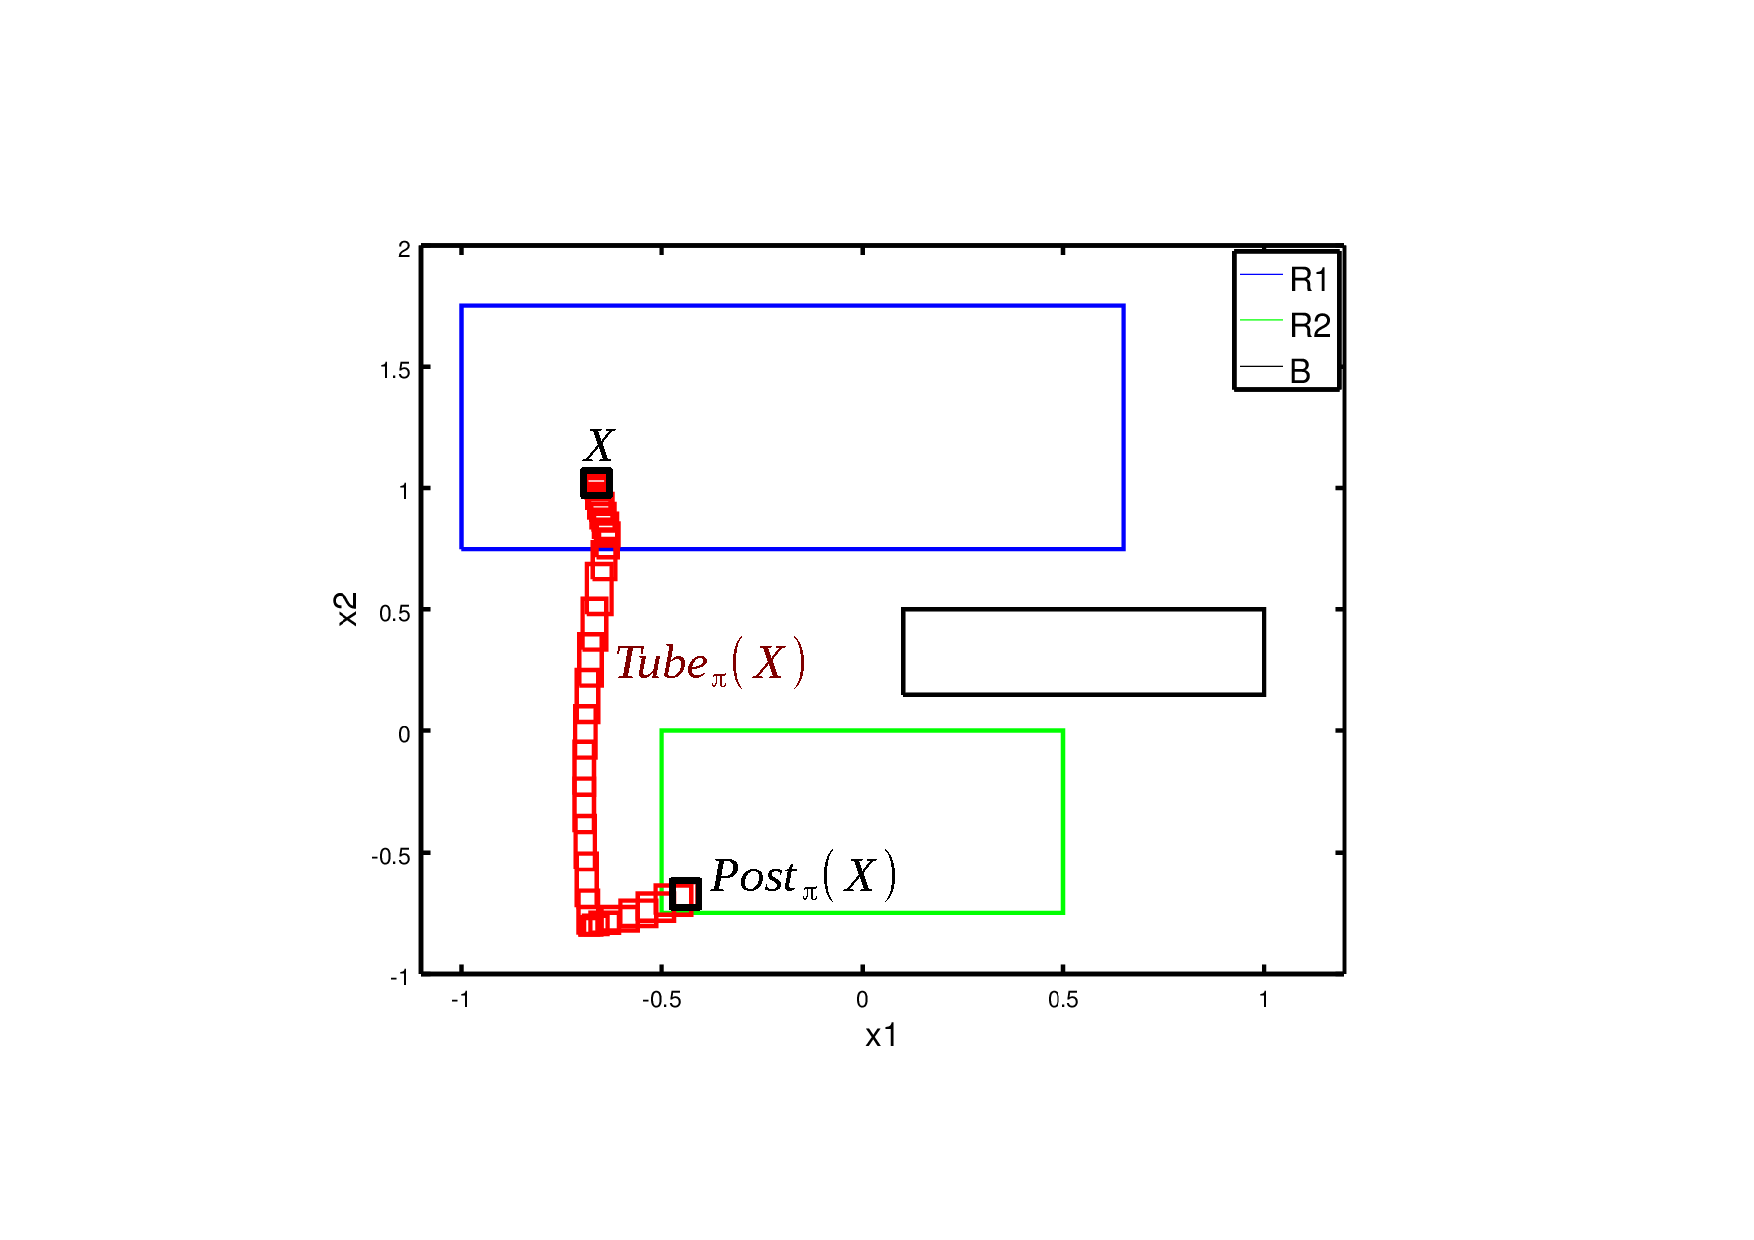
\includegraphics[trim = 4cm 3cm 4cm 4cm, clip,
width=0.5\textwidth]{tube.pdf}
 \caption{Functions $Post_{\pi}(X)$ and $Tube_{\pi}(X)$ for the
   initial box $X=[-0.69,-0.64] \times [1,1.06]$, with a pattern $\pi
   = (1,3,0)$.}
 \label{fig:post_illustration}
\end{figure}


\section{General principle}

We introduce a first basic procedure permitting to perform $(R,S)$-stability, and 
omit the perturbation in a first time.
Given a set $R$, let $\{W_i\}_{i \in I}$ be a family of 
sets such that $R \subseteq \bigcup_{i \in I} W_i \subseteq S$ as illustrated
in Figure \ref{fig:covering}.
If one can find, for each $W_i$ for $i \in I$, a pattern $\pi_i$
such that $Post_{\pi_i} (W_i) \subseteq R$, then we can induce 
an infinite-time switching rule permitting
to return infinitely often in $R$.


\begin{figure}[h]
\centering
 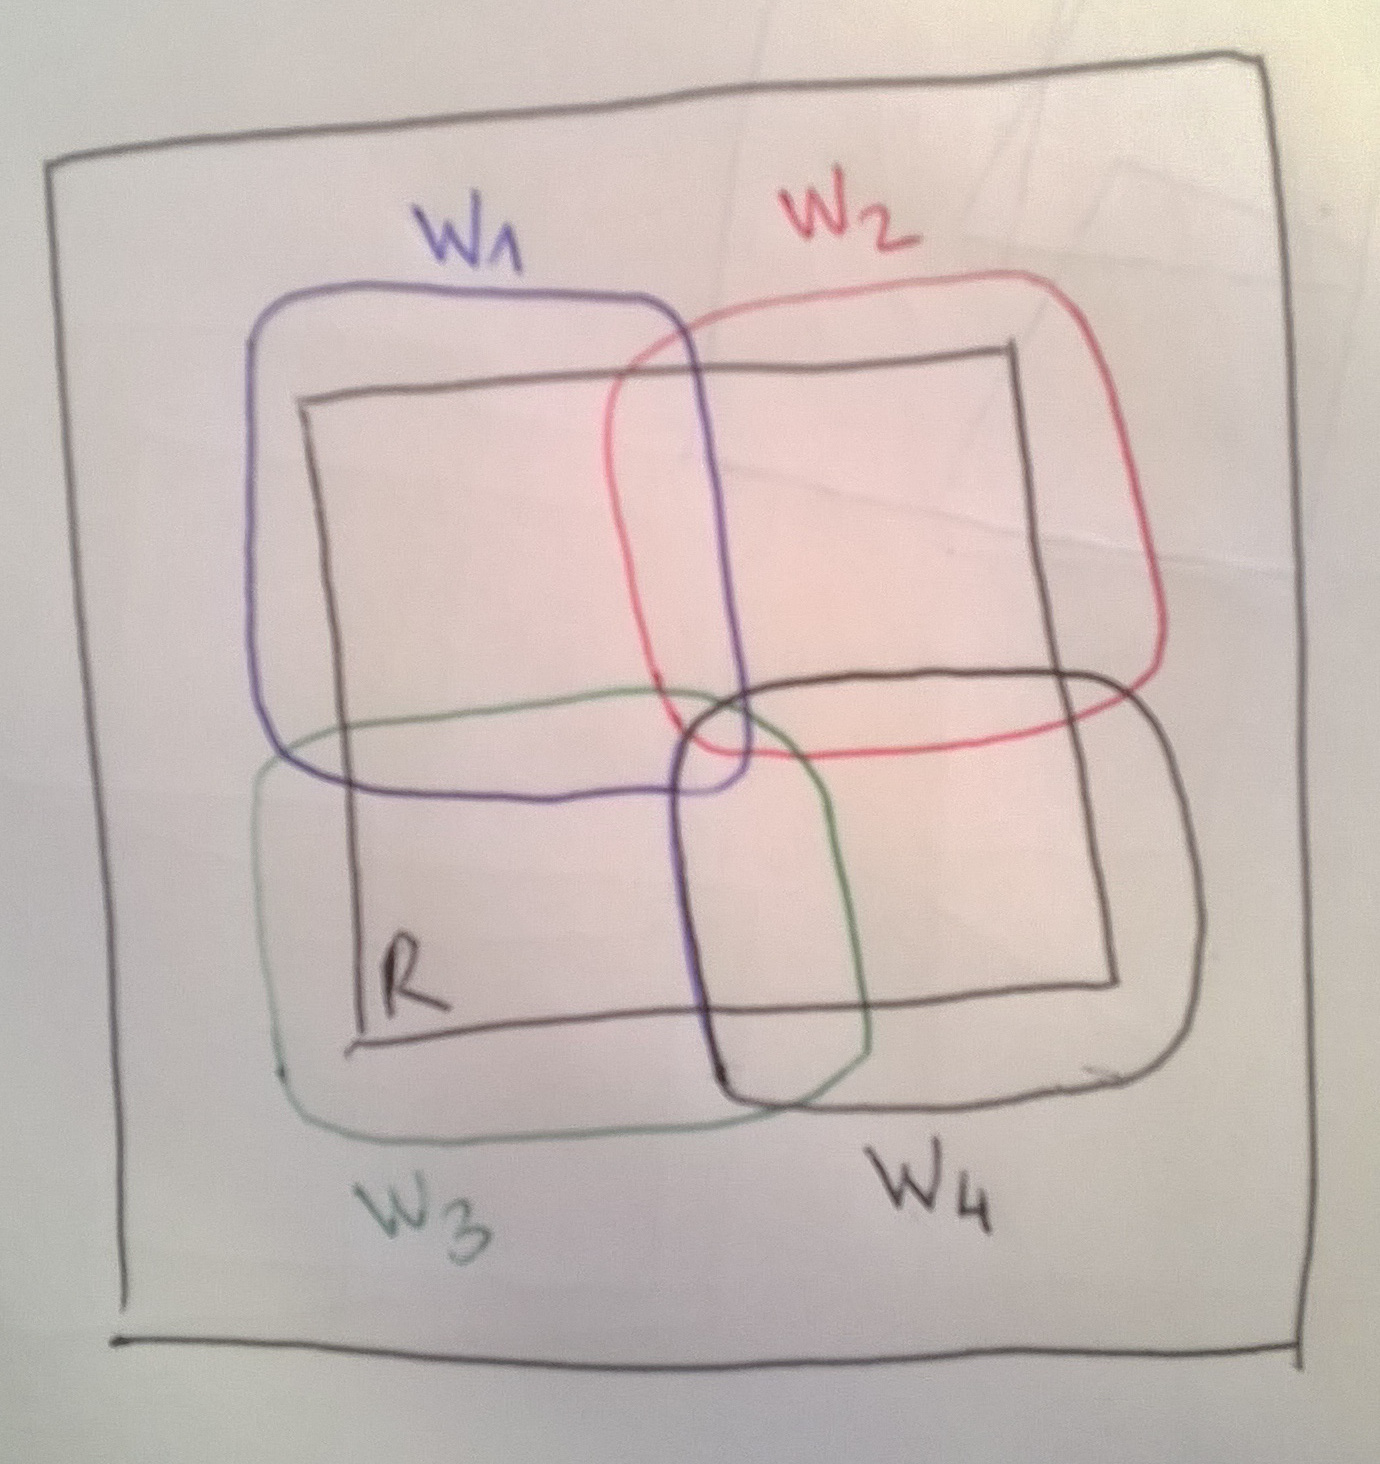
\includegraphics[scale=0.15]{covering.jpg}
 \label{fig:covering}
 \caption{A family of sets covering $R$.}
\end{figure}

\begin{theorem}
 Let $R \subseteq \R^n$, suppose we are given a
 switched system satisfying \eqref{eq:switched_system0}.
 A family of sets $\{W_i\}_{i \in I}$ associated to 
 patterns $\{\pi_i\}_{i \in I}$
 such that 
 \begin{itemize}
  \item $R \subseteq \bigcup_{i \in I} W_i \subseteq S$ 
  \item  for all $i \in I$, $Post_{\pi_i} (W_i) \subseteq R$
 \end{itemize}
 induces an infinite-time control ensuring recurrence in $R$. 
 \label{th:R-procedure}
\end{theorem}
\begin{proof}
 Let $x_0 \in R$, there exists $i_0 \in I$ such that $x_0 \in W_{i_0}$ since 
 $R \subseteq \bigcup_{i \in I} W_i$. Application of pattern 
 $\pi_{i_0}$ leads to a state $x_1 = \phi( \tau;0,x_0,\pi_{i_0})$
 also belonging to $R$ since $Post_{\pi_{i_0}}(W_{i_0}) \subseteq R$. State $x_1$
 thus belongs to $W_{i_1}$ for some $i_1 \in I$, and by recurrence, 
 one can obtain a sequence of points $x_0,x_1,\dots$ all belonging to 
 $R$. The induced trajectory thus returns infinitely often in $R$.
\end{proof}

A simple extension of this procedure, relying on the computation
of reachability tubes, allows to ensure safety in $S \subseteq \R^n$ as follows.

\begin{theorem}
 Let $R \subseteq \R^n$, $S \subseteq \R^n$, suppose we are given a
 switched system satisfying \eqref{eq:switched_system0}.
 A family of sets $\{W_i\}_{i \in I}$ associated to 
 patterns $\{\pi_i\}_{i \in I}$
 such that 
 \begin{itemize}
  \item $R \subseteq \bigcup_{i \in I} W_i \subseteq S$ 
  \item  for all $i \in I$, $Post_{\pi_i} (W_i) \subseteq R$
  \item  for all $i \in I$, $Tube_{\pi_i} (W_i) \subseteq S$
  \end{itemize}
 induces an infinite-time control ensuring recurrence in $R$ and safety in $S$. 
 \label{th:RS-procedure}
\end{theorem}
\begin{proof}
The recurrence in $R$ is proved with the same arguments as the proof 
of Theorem~\ref{th:R-procedure}. The safety in $S$ is ensured 
by the definition of $Tube_{\pi_i}(W_i)$, with permits 
to ensure that for all $x_0 \in R$, $i \in I$, $t \in k_i\tau$, where $k_i$
is the length of pattern $\pi_i$, we have
$\phi( t;0,x_0,\pi_{i}) \in S$.
\end{proof}

Having defined the principle of the procedure, we now present 
how controllers can be numerically computed 
using Theorem \ref{th:R-procedure} and \ref{th:RS-procedure}.
At this point, two main problems arise. The first is the construction
of a family $\{W_i\}_{i \in I}$ covering $R$, the second 
is ensuring that for all $i \in I$, $Post_{\pi_i} (W_i) \subseteq R$ and
$Tube_{\pi_i} (W_i) \subseteq S$.
The first problem can be solved using heuristics, but depends of 
the type of sets one uses, the second is actually impossible to ensure exactly, in the 
sense that solutions of ODEs are not known in general (particularly 
when the initial condition is a set).
Supposing that one can compute reachability sets and tubes, the procedure works
as follows in practice. First, we generate a coarse covering 
of $R$ (starting for example by considering the whole set $R$), 
we then try to compute patterns associated to each set of 
the covering. If this last step fails, we generate another finer tiling, performing 
for example a bisection of each dimension of $R$, and one now has to control
each bisected part of $R$.
This is a simple heuristics, but which works well in practice (as seen in the following Sections ???).
In the following, we use a uniform covering of $R$ with boxes and balls of $\R^n$. If each box or ball
is controlled, the problem is solved, otherwise, we use a finer covering. 
We address the problem of computing reachability sets and tubes in the following chapters.
% and introduce some hypotheses for this purpose.
We now present in details the possible heuristics and associated algorithms 
for control synthesis, supposing that one can compute 
the Post and Tube operators.

% We now introduce an algorithm for the recurrence only property in $R$,
% using zonotope transformations for linear systems,
% in association with a heuristics decomposing $R$. It showed to be very efficient 
% for practical use for linear systems, but unfortunately cannot guarantee safety between 
% time steps for continuous systems. However, if the system is formulated 
% in a discrete time form, formal guarantees of safety can be ensured.
% The algorithm is composed of two main functions, given in Algorithm \ref{algo:basic_decomposition}
% and \ref{algo:basic_findpat}.

% \begin{algorithm}
%   \centering
%   \begin{algorithmic}
%     \STATE{\textbf{Function:} $Decomposition(W,R,D,K)$}
%     \STATE{\begin{center}\line(1,0){150}\end{center}}
%     \STATE{\quad \textbf{Input:} A box $W$, a box $R$, a degree $D$ of bisection,
%       a length $K$ of input pattern}\STATE{\quad \textbf{Output:}$\langle\{(V_i,\pi_i)\}_{i},True\rangle$ or $\langle\_ ,False\rangle$}
%     \STATE{\begin{center}\line(1,0){150}\end{center}}
%     \STATE{ $(\pi,b) := Find\_Pattern(W,R,K)$}
%     \IF{$b=True$}{
%       \STATE{\textbf{return} $\langle\{(W,Pat)\},True\rangle$}
%     }
%     \ELSE
%     \IF{$D = 0$} \RETURN{$\langle \_,False\rangle$} \ELSE
%     \STATE{Divide equally $W$ into $(W_1, W_{2})$ \FOR{$i=1,2$}\STATE{\small{$(\Delta_i,b_i)$ := $Decomposition(W_i,R,D - 1,K)$}}\ENDFOR
%       \RETURN $(\bigcup_{i=1,2} \Delta_i,\bigwedge_{i=1,2} b_i)$ } \ENDIF
%     \ENDIF
%   \end{algorithmic}
%   \caption{Algorithmic form of Function $Decomposition$.}
%   \label{algo:basic_decomposition}
% \end{algorithm}
% 
% 
% 
% \begin{algorithm}[t]
%   \centering
%   \begin{algorithmic}
%     \STATE{\textbf{Function:} $Find\_Pattern(W,R,K)$}
%     \STATE{\begin{center}\line(1,0){150}\end{center}}
%     \STATE{\quad \textbf{Input:}A box $W$, a box $R$, a length $K$ of input pattern}
%     \STATE{\quad \textbf{Output:}$\langle \pi,True\rangle$ or $\langle\_, False\rangle$}
%     \STATE{\begin{center}\line(1,0){150}\end{center}}
%     \FOR{$i=1\dots K$} \STATE{$\Pi :=$ set of input patterns of length $i$}
%     \WHILE{$\Pi$ is non empty} \STATE{Select $\pi$ in $\Pi$}
%     \STATE{$\Pi:= \Pi\setminus  \{\pi\}$}
%     \IF{$Post_{\pi}(W) \subseteq R$}{\RETURN{$\langle \pi,True\rangle$}} \ENDIF
%     \ENDWHILE
%     \ENDFOR
%     \RETURN{$\langle \_,False \rangle$}
%   \end{algorithmic}
%   \caption{Algorithmic form of Function $Find\_Pattern$.}
%   \label{algo:basic_findpat}
% \end{algorithm}


\subsection{The state-space bisection algorithm}
\label{sec:minimator}

% \subsubsection{Principle of the algorithm}

We describe the algorithm solving the control synthesis problem for
nonlinear switched systems (see Problem~\ref{prob:nl_control},
Section~\ref{sec:intro_detailed}). Given the input boxes $R$, $S$, $B$, and
given two positive integers $K$ and $D$, the algorithm provides, when
it succeeds, a decomposition $\Delta$ of $R$ of the form $\{ V_i,
\pi_i \}_{i \in I}$, with the properties:
\begin{itemize}
\item $\bigcup_{i \in I} V_i = R$,
\item $\forall i \in I, \ Post_{\pi_i}(V_i) \subseteq R$,
\item $\forall i \in I, \ Tube_{\pi_i}(V_i) \subseteq S$,
\item $\forall i \in I, \ Tube_{\pi_i}(V_i) \bigcap B = \emptyset$.
\end{itemize}

The sub-boxes $\{ V_i \}_{i \in I}$ are obtained by repeated
bisection.  At first, function $Decomposition$ calls sub-function
$Find\_Pattern$ which looks for a pattern $\pi$ of length at most $K$
such that $Post_{\pi}(R) \subseteq R$, $Tube_{\pi}(R) \subseteq S$ and
$Tube_{\pi}(R) \bigcap B = \emptyset$.  If such a pattern $\pi$ is
found, then a uniform control over $R$ is found (see
Figure~\ref{fig:scheme}(a)). Otherwise, $R$ is divided into two
sub-boxes $V_1$, $V_{2}$, by bisecting $R$ w.r.t. its longest
dimension. Patterns are then searched to control these sub-boxes (see
Figure~\ref{fig:scheme}(b)). If for each $V_i$, function
$Find\_Pattern$ manages to get a pattern $\pi_i$ of length at most $K$
verifying $Post_{\pi_i}(V_i) \subseteq R$, $Tube_{\pi_i}(V_i)
\subseteq S$ and $Tube_{\pi_i}(V_i) \bigcap B = \emptyset$, then it is
a success and algorithm stops.  If, for some $V_j$, no such pattern is
found, the procedure is recursively applied to $V_j$.  It ends with
success when every sub-box of $R$ has a pattern verifying the latter
conditions, or fails when the maximal degree of decomposition $D$ is
reached.  The algorithmic form of functions $Decomposition$ and
$Find\_Pattern$ are given in Algorithm~\ref{algo:decomposition} and
Algorithm~\ref{algo:findpattern} respectively. Note that a special form
of Algorithm~\ref{algo:findpattern} for linear ODEs can be found
in~\cite{fribourg2014finite}.

\begin{figure}[ht]
 \centering
 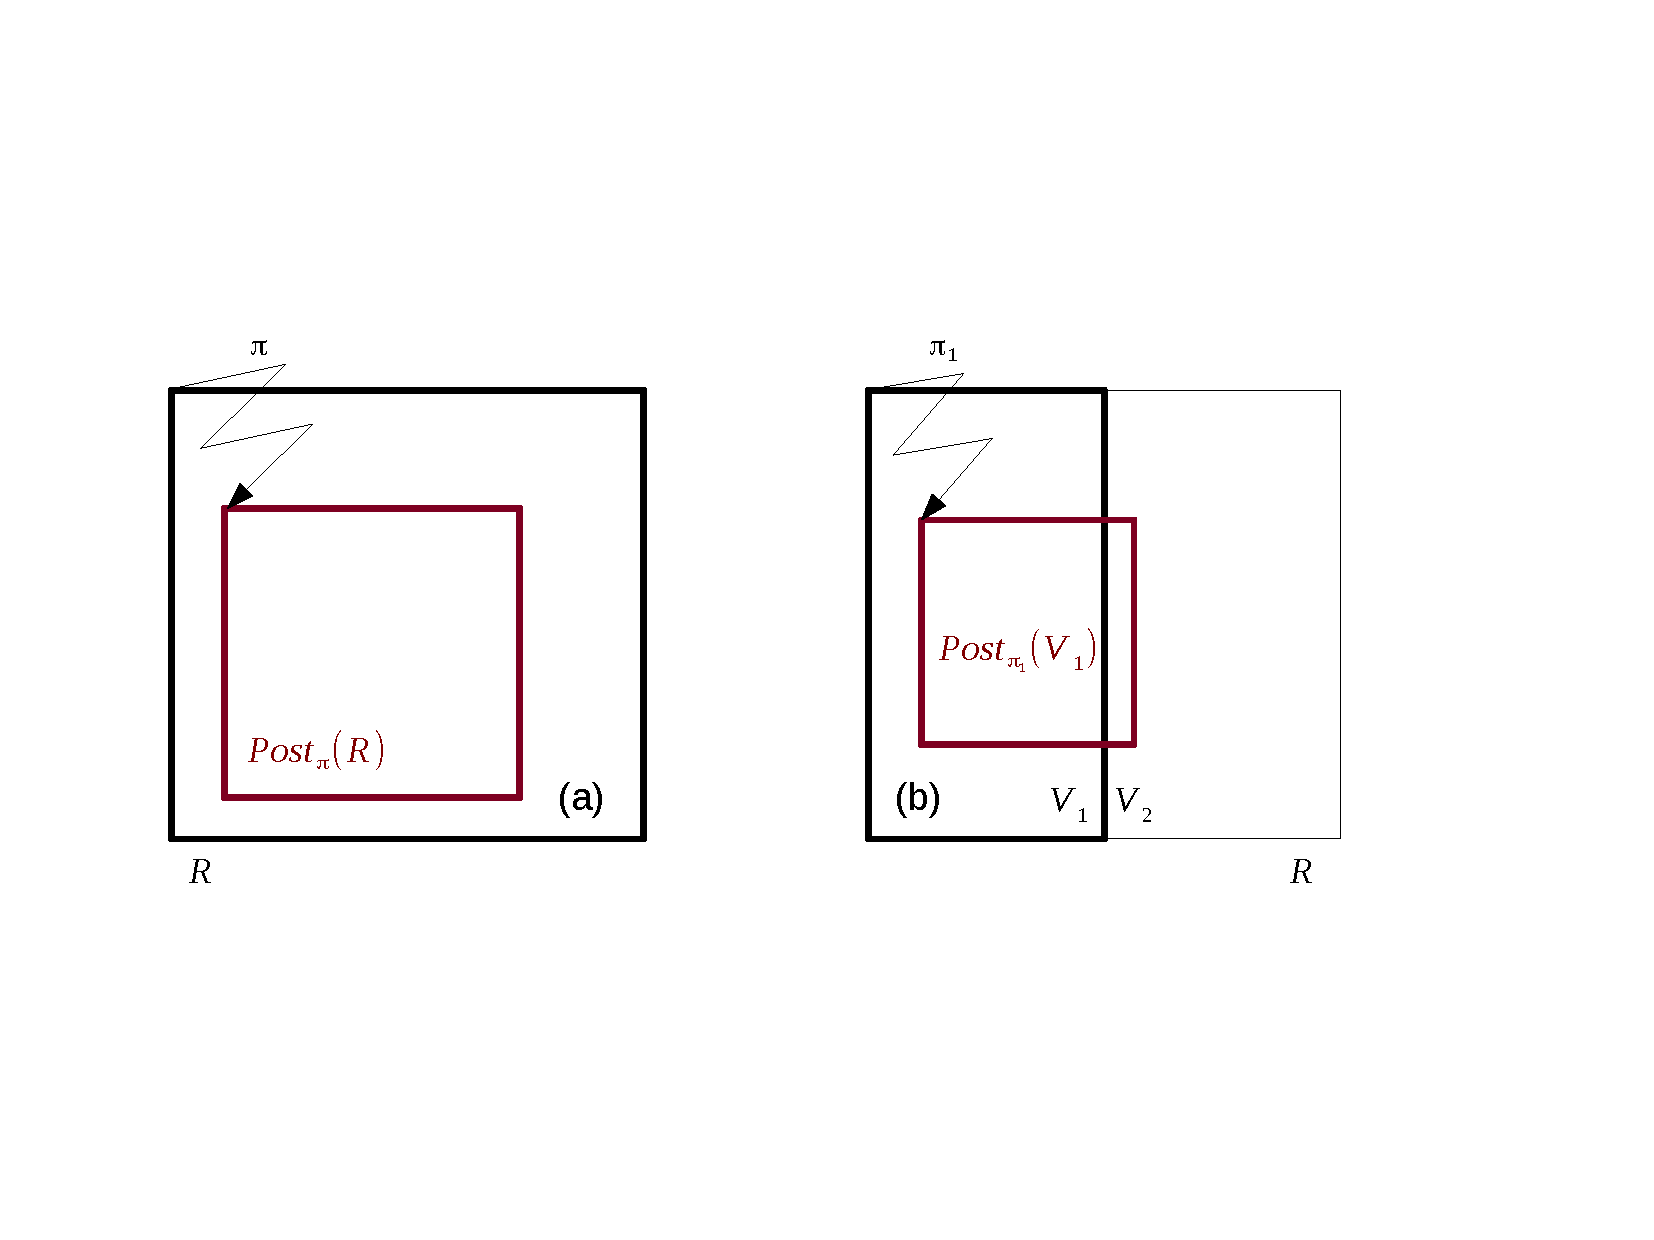
\includegraphics[%trim = 2cm 6cm 4cm 5.5cm, clip,
 width=0.6\textwidth]{bisect.pdf}
 \caption{Principle of the bisection method.}
 \label{fig:scheme}
\end{figure}


\begin{algorithm}
  \centering
  \begin{algorithmic}
    \STATE{\textbf{Function:} $Decomposition(W,R,S,B,D,K)$}
    \STATE{\begin{center}\line(1,0){150}\end{center}}
    \STATE{\quad \textbf{Input:} A box $W$, a box $R$, a box $S$, a box $B$, a degree $D$ of bisection,
      a length $K$ of input pattern}\STATE{\quad \textbf{Output:}$\langle\{(V_i,\pi_i)\}_{i},True\rangle$ or $\langle\_ ,False\rangle$}
    \STATE{\begin{center}\line(1,0){150}\end{center}}
    \STATE{ $(\pi,b) := Find\_Pattern(W,R,S,B,K)$}
    \IF{$b=True$}{
      \STATE{\textbf{return} $\langle\{(W,Pat)\},True\rangle$}
    }
    \ELSE
    \IF{$D = 0$} \RETURN{$\langle \_,False\rangle$} \ELSE
    \STATE{Divide equally $W$ into $(W_1, W_{2})$ \FOR{$i=1,2$}\STATE{\small{$(\Delta_i,b_i)$ := $Decomposition(W_i,R,S,B,D - 1,K)$}}\ENDFOR
      \RETURN $(\bigcup_{i=1,2} \Delta_i,\bigwedge_{i=1,2} b_i)$ } \ENDIF
    \ENDIF
  \end{algorithmic}
  \caption{Algorithmic form of Function $Decomposition$.}
  \label{algo:decomposition}
\end{algorithm}


Our control synthesis method being well defined, we introduce the main
result of this section, stated as follows:
 \begin{proposition}
   Algorithm~\ref{algo:decomposition} with input
   $(R,R,S,B,D,K)$ returns, when it successfully terminates, a
   decomposition $\{ V_i,\pi_i \}_{i \in I}$ of~$R$ which solves
   Problem~\ref{prob:nl_control}.
 \end{proposition}
%
 \begin{proof}
   Let $x_0 = x(t_0=0)$ be an initial condition belonging to~$R$. If
   the decomposition has terminated successfully, we have $\bigcup_{i
     \in I} V_i = R$, and $x_0$ thus belongs to $V_{i_0}$ for some
   $i_0\in I$.  We can thus apply the pattern $\pi_{i_0}$ associated
   to $V_{i_0}$. Let us denote by $k_0$ the length of $\pi_{i_0}$. We
   have:
   \begin{itemize}
   \item $\phi_{\pi_{i_0}}(k_0\tau;0,x_0,d) \in R$
   \item $\forall t \in [0, k_0\tau], \quad
     \phi_{\pi_{i_0}}(t;0,x_0,d) \in S$
   \item $\forall t \in [0, k_0\tau], \quad
     \phi_{\pi_{i_0}}(t;0,x_0,d) \notin B$
   \end{itemize}
   Let $x_1 = \phi_{\pi_{i_0}}(k_0\tau;0,x_0,d) \in R$ be the
   state reached after application of $\pi_{i_0}$ and let $t_1 = k_0
   \tau$.  State $x_1$ belongs to $R$, it thus belongs to $V_{i_1}$
   for some $i_1 \in I$, and we can apply the associated pattern
   $\pi_{i_1}$ of length $k_1$, leading to:
   \begin{itemize}
   \item $\phi_{\pi_{i_1}}(t_1 + k_1\tau;t_1,x_1,d) \in R$
   \item $\forall t \in [t_1, t_1 + k_1\tau], \quad
     \phi_{\pi_{i_1}}(t;t_1,x_1,d) \in S$
   \item $\forall t \in [t_1, t_1 + k_1\tau], \quad
     \phi_{\pi_{i_1}}(t;t_1,x_1,d) \notin B$
   \end{itemize}
   We can then iterate this procedure from the new state
   \begin{displaymath}
     x_2 =
     \phi_{\pi_{i_1}}(t_1 + k_1\tau;t_1,x_1,d) \in R.
   \end{displaymath}
   This can be repeated infinitely, yielding a sequence of points
   belonging to $R$ $x_0,x_1,x_2,\dots$ attained at times
   $t_0,t_1,t_2,\dots$, when the patterns
   $\pi_{i_0},\pi_{i_1},\pi_{i_2},\dots$ are applied.

   We furthermore have that all the trajectories stay in $S$ and never
   cross $B$:
   \begin{displaymath}
     \forall t \in \mathbb{R}^+, \exists k \geq 0, \ t \in
     \lbrack t_k , t_{k+1} \rbrack
   \end{displaymath}
   and
   \begin{displaymath}
     \forall t \in \lbrack t_k ,
     t_{k+1} \rbrack,\ \phi_{\pi_{i_k}} ( t; t_k, x_k, d) \in S,\
     \phi_{\pi_{i_k}} (t;t_k, x_k, d) \notin B .
   \end{displaymath}
   The trajectories thus return infinitely often in $R$, while always
   staying in $S$ and never crossing $B$.
\end{proof}

 \begin{remark}
   Note that it is possible to perform reachability from a set $R_1$
   to another set $R_2$ by computing $Decomposition(R_1,R_2,S,B,D,K)$.
   The set $R_1$ is thus decomposed with the objective to send its
   sub-boxes into $R_2$, \textit{i.e.}, for a sub-box $V$ of $R_1$,
   patterns $\pi$ are searched with the objective $Post_{\pi}(V)
   \subseteq R_2$ (see Example~\ref{ex2}).
 \end{remark}

\begin{algorithm}[t]
  \centering
  \begin{algorithmic}
    \STATE{\textbf{Function:} $Find\_Pattern(W,R,S,B,K)$}
    \STATE{\begin{center}\line(1,0){150}\end{center}}
    \STATE{\quad \textbf{Input:}A box $W$, a box $R$, a box $S$, a box $B$, a length $K$ of input pattern}
    \STATE{\quad \textbf{Output:}$\langle \pi,True\rangle$ or $\langle\_, False\rangle$}
    \STATE{\begin{center}\line(1,0){150}\end{center}}
    \FOR{$i=1\dots K$} \STATE{$\Pi :=$ set of input patterns of length $i$}
    \WHILE{$\Pi$ is non empty} \STATE{Select $\pi$ in $\Pi$}
    \STATE{$\Pi:= \Pi\setminus  \{\pi\}$}
    \IF{$Post_{\pi}(W) \subseteq R$ \AND $Tube_{\pi}(W) \subseteq S$ \AND $Tube_{\pi}(W) \bigcap B = \emptyset$ }{\RETURN{$\langle \pi,True\rangle$}} \ENDIF
    \ENDWHILE
    \ENDFOR
    \RETURN{$\langle \_,False \rangle$}
  \end{algorithmic}
  \caption{Algorithmic form of Function $Find\_Pattern$.}
  \label{algo:findpattern}
\end{algorithm}


In Algorithm \ref{algo:decomposition} and \ref{algo:findpattern}, 
we use a bisection of uncontrolled tiles into two parts (by bisecting the greatest 
dimension). But another possible heuristics is to divide 
uncontrolled parts into $2^n$ parts, by bisecting each dimension. 
This leads to a faster growing of the number of tiles to be controlled, but 
can sometimes lead to lower computation times, when the system requires a fine tiling. 
The two possible heuristics are schemed in Figure \ref{fig:heuristics}. 

\begin{figure}
\centering
 \begin{tabular}{cc}
  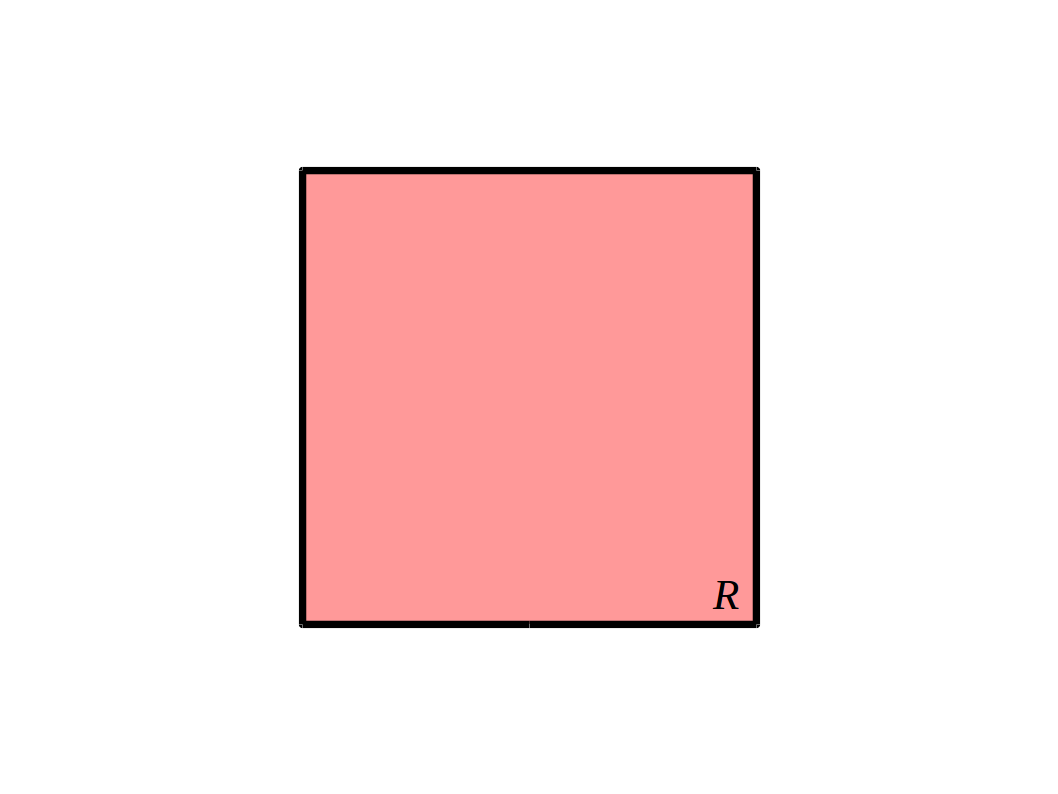
\includegraphics[width=0.4\textwidth]{tiling_R_heuristics102.png} &   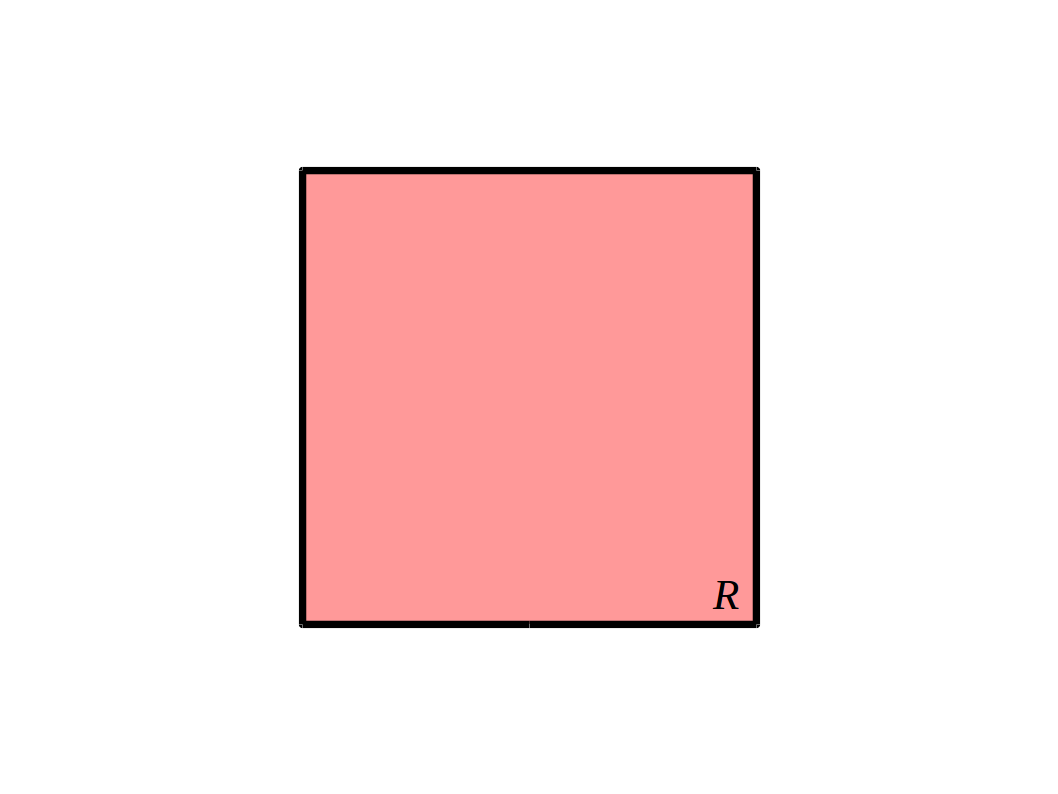
\includegraphics[width=0.4\textwidth]{tiling_R_heuristics102.png} \\
  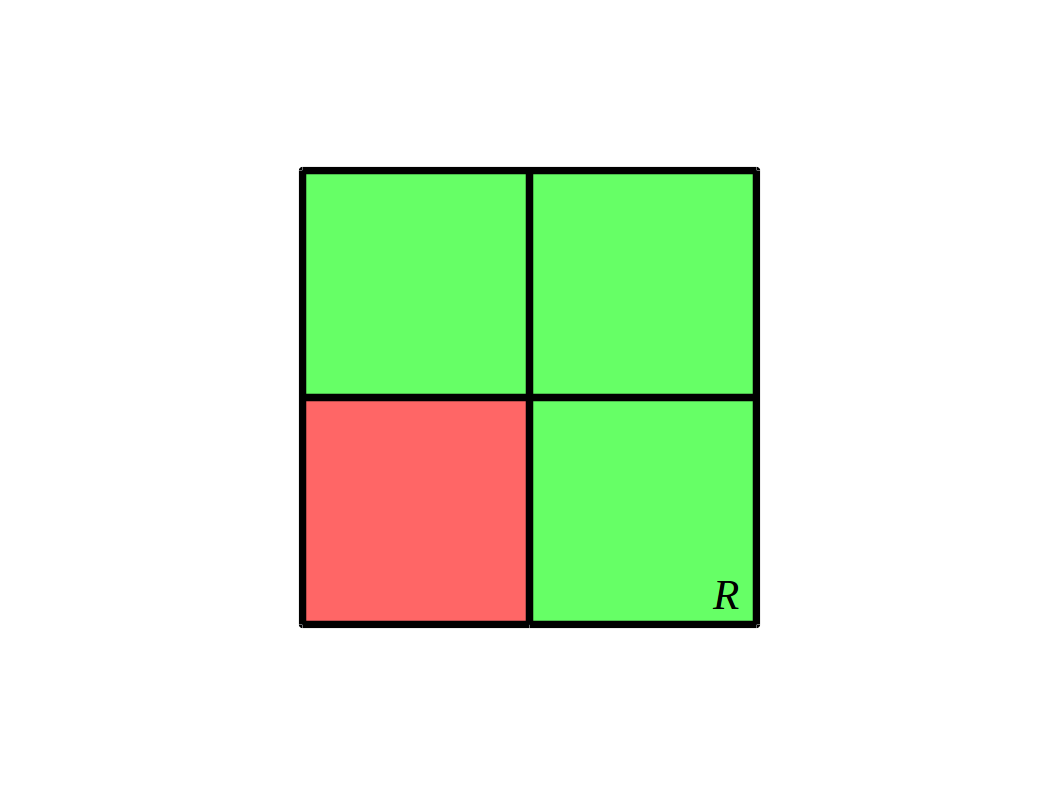
\includegraphics[width=0.4\textwidth]{tiling_R_heuristics112.png} &   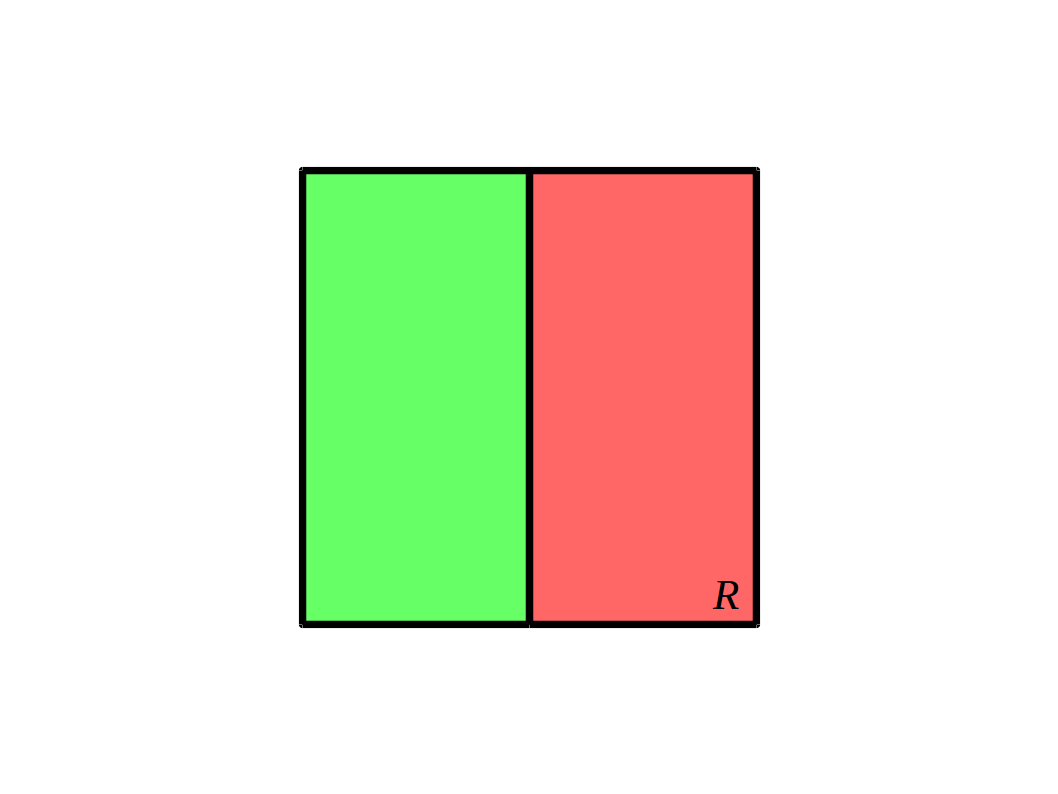
\includegraphics[width=0.4\textwidth]{tiling_R_heuristics212.png} \\  
  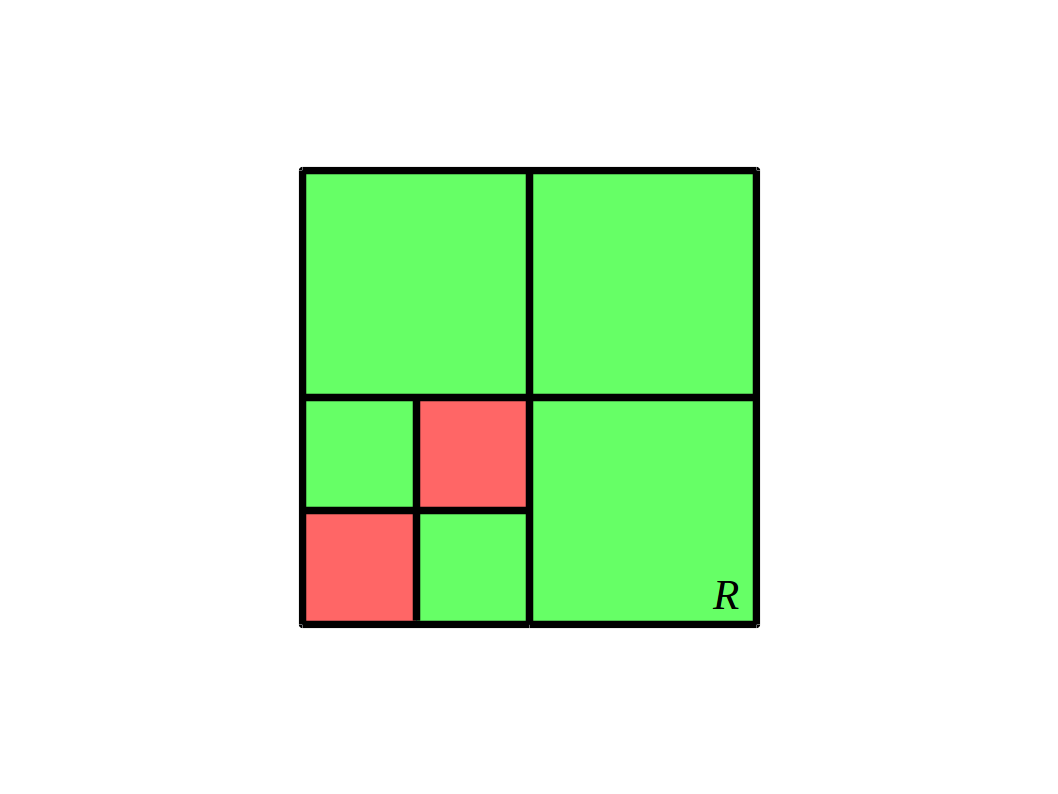
\includegraphics[width=0.4\textwidth]{tiling_R_heuristics122.png} &   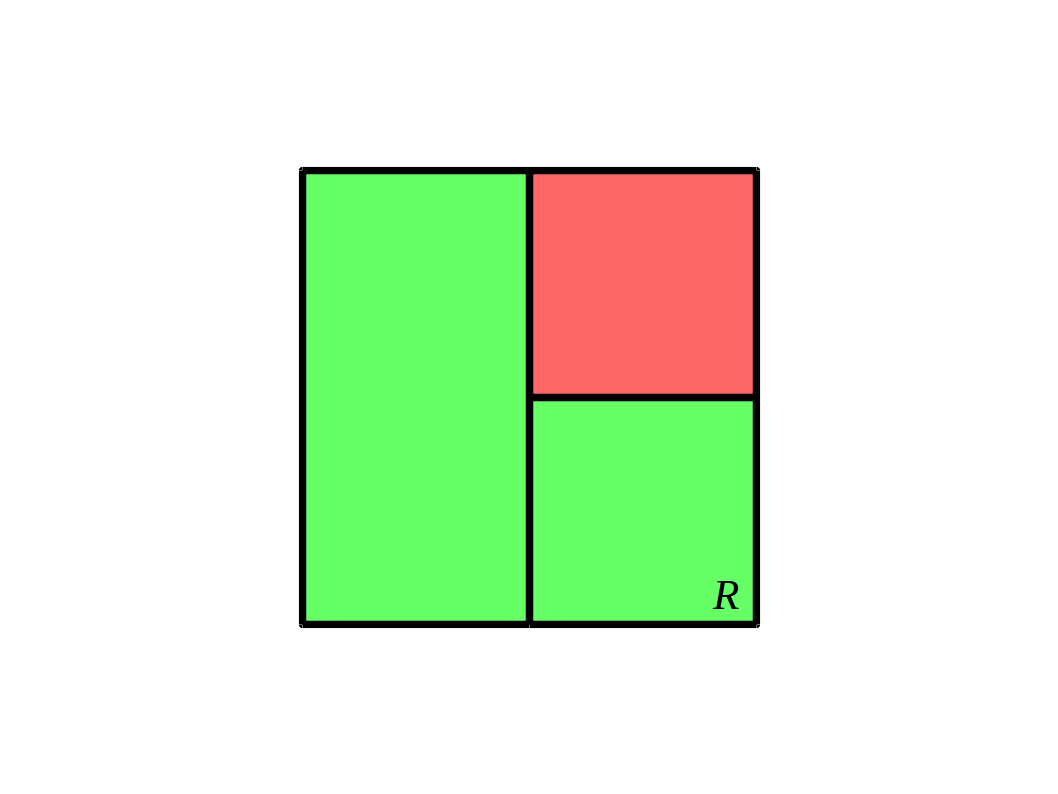
\includegraphics[width=0.4\textwidth]{tiling_R_heuristics222.png} \\  
  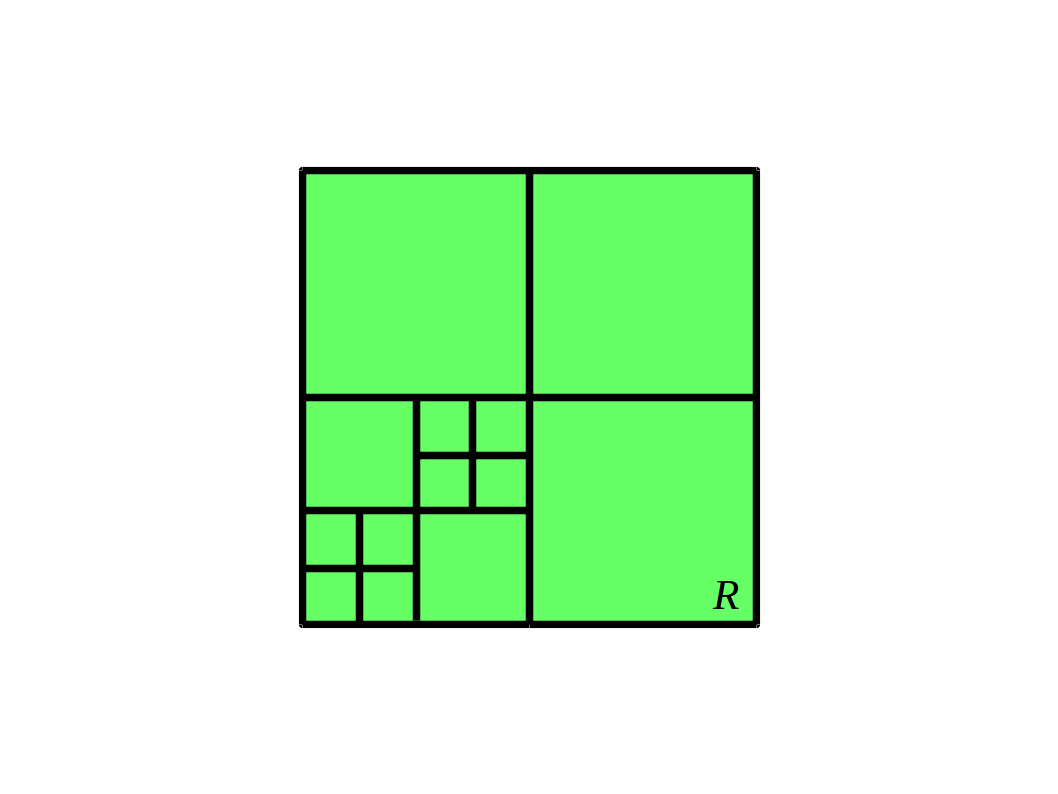
\includegraphics[width=0.4\textwidth]{tiling_R_heuristics132.png} &   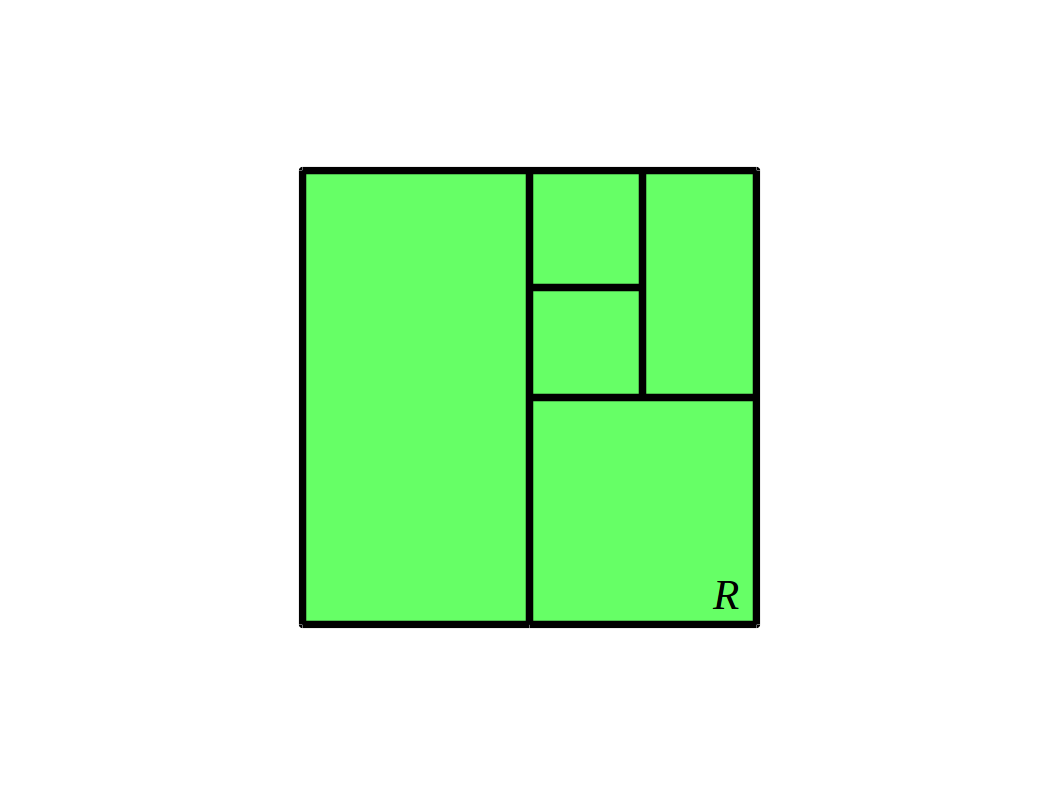
\includegraphics[width=0.4\textwidth]{tiling_R_heuristics242.png} \\  
  \end{tabular}
 \caption{Scheme of the two possible heuristics: green 
tiles have been controlled (associated to a pattern), and red tiles have yet to be controlled and
bisected. Left: bisection of all the dimensions; right: bisection of the largest dimension}
\label{fig:heuristics}
\end{figure}


  \subsection{A covering of balls}

  So far, we used boxes of $\R^n$ to represent sets of states.
  Balls of $\R^n$ are actually another useful way of representing it, since we provide 
  an efficient way of performing reachability analysis with such sets (see Chapter \ref{chap:1}).
  A covering of $R$ can be performed as schemed in Figure \ref{fig:tilingball}.
  Let $\delta$ be a radius, each set $W_i = B(\tilde x_i, \delta)$ has to be controlled, otherwise,
  a fined covering (using more balls) should be used.
  Actually, the same heuristics as boxes could be used, since these balls 
  can be built as circumscribed balls of the boxes.
  
  
  
  \begin{figure}
  \centering
   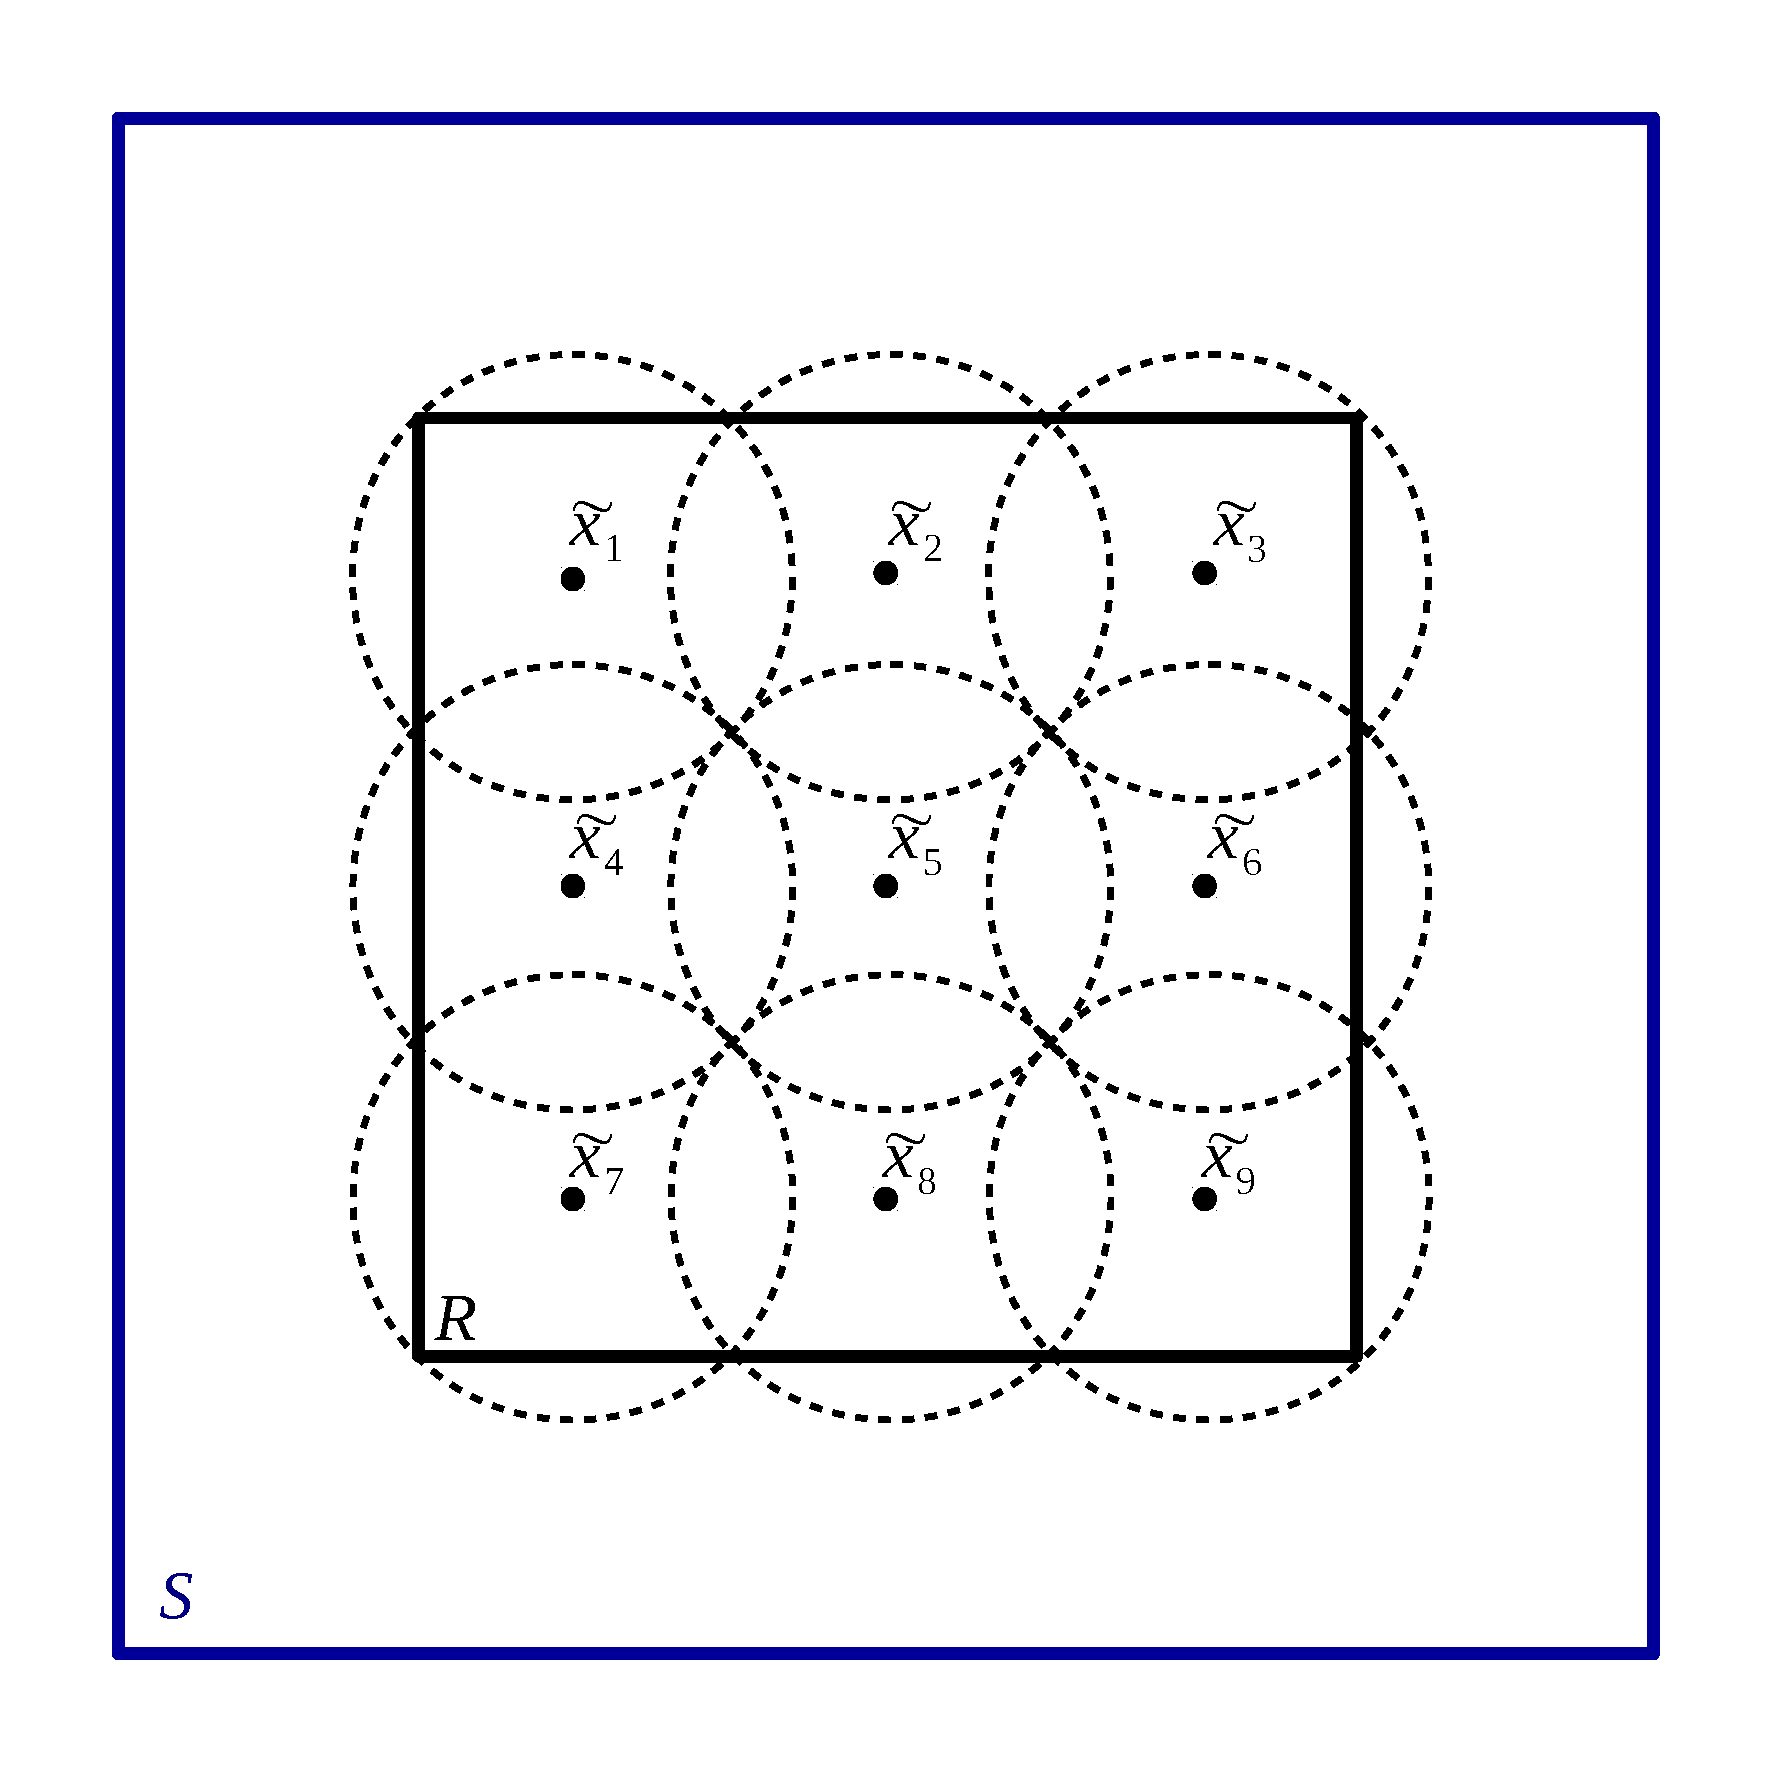
\includegraphics[width=0.5\textwidth]{tilingball2.pdf}
   \caption{Scheme of a covering of $R \subset \R^2$ with balls.}
   \label{fig:tilingball}
  \end{figure}

  
 \subsection{Improving the research of patterns}
%
 We propose in this section an improvement of the function
 $Find\_Pattern$ given in~\cite{NL_minimator,fribourg2014finite},
 which is a naive testing of all the patterns of growing length (up to
 $K$).


 \begin{algorithm}[t]
   \centering
   \begin{algorithmic}
     \STATE{\textbf{Function:} $Find\_Pattern2(W,R,S,B,K)$}
     \STATE{\begin{center}\line(1,0){150}\end{center}}
     \STATE{\quad \textbf{Input:}A box $W$, a box $R$, a box $S$, a box $B$, a length $K$ of input pattern}
     \STATE{\quad \textbf{Output:}$\langle \pi,True\rangle$ or $\langle\_, False\rangle$}
     \STATE{\begin{center}\line(1,0){150}\end{center}}

     \STATE{$\mathcal{S} = \{  \emptyset \}$}
     \STATE{$\mathcal{L} = \{ \left(W,W, \emptyset \right) \}$}
     \WHILE{$\mathcal{L} \neq \emptyset$} \STATE{$e_{\text{current}}$ = takeHead($\mathcal{L}$)}

 \FOR{$i \in U$}
    \IF{$Post_{i}(e_{\text{current}}.Y_{\text{current}}) \subseteq R$ \AND $Tube_{i}(e_{\text{current}}.{Y_{\text{current}}}) \bigcap B = \emptyset$ \AND $Tube_{i}(e_{\text{current}}.Y_{\text{current}}) \subseteq S$} \STATE{$\text{putTail}(\mathcal{S},e_{\text{current}}.\Pi + i)$ {\color{blue} /* or also ``{\bf return} $\langle e_{\text{current}}.\Pi + i,True \rangle$'' */ } }
  \ELSE{ \IF{$Tube_{i}(e_{\text{current}}.{Y_{\text{current}}}) \bigcap B \neq \emptyset$ \OR
      $Tube_{i}(e_{\text{current}}.{Y_{\text{current}}}) \nsubseteq S$} \STATE{ discard $e_{\text{current}}$ } \ENDIF}
    \ELSE{ \IF{$Tube_{i}(e_{\text{current}}.{Y_{\text{current}}}) \bigcap B = \emptyset$ \AND $Tube_{i}(e_{\text{current}}.Y_{\text{current}}) \subseteq S$}
      \STATE{\IF{$\text{Length}(\Pi)+1 < K$} \STATE{$\text{putTail}(\mathcal{L},\left(e_{\text{current}}.Y_{\text{init}}, Post_i(e_{\text{current}}.Y_{\text{current}}),e_{\text{current}}.\Pi + i \right))$ }   \ENDIF} \ENDIF}

    \ENDIF
  \ENDFOR
 \ENDWHILE

 \RETURN{$\langle \_,False \rangle$ if no solution is found, or $\langle \pi,True\rangle$, $\pi$ being
 any pattern validated in $Solution$.}
 \end{algorithmic}
\caption{Algorithmic form of Function $Find\_Pattern2$.}
\label{algo:findpattern2}
\end{algorithm}


 The improved function, denoted here by $Find\_Pattern2$, exploits
 heuristics to prune the search tree of patterns. We present it
 with boxes of $\R^n$, but can also be used with balls. The algorithmic form
 of $Find\_Pattern2$ is given in Algorithm~\ref{algo:findpattern2}.  It
 relies on a new data structure consisting of a list of triplets
 containing:
 \begin{itemize}
 \item An initial box $V \subset \mathbb{R}^n$,
  \item A {\em current} box $Post_{\pi}(V)$, image of $V$ by the pattern $\pi$,
  \item The associated pattern $\pi$.
 \end{itemize}
 For any element $e$ of a list of this type, we denote by $e.Y_{\text{init}}$
 the initial box, $e.Y_{\text{current}}$ the {\em current} box, and by
 $e.\Pi$ the associated pattern.  We denote by $e_{\text{current}} =
 takeHead(\mathcal{L})$ the element on top of a list $\mathcal L$
 (this element is removed from list $\mathcal L$).  The function
 $putTail(\cdot,\mathcal{L})$ adds an element at the end of the list
 $\mathcal L$.

 Let us suppose one wants to control a box $X \subseteq R$.  The list
 $\mathcal{L}$ of Algorithm~\ref{algo:findpattern2} is used to store the
 intermediate computations leading to possible solutions (patterns
 sending $X$ in $R$ while never crossing $B$ or $\mathbb{R}^n
 \setminus S$). It is initialized as $\mathcal{L} = \{ \left(X,X,
   \emptyset \right) \}$.  First, a testing of all the control modes
 is performed (a set simulation starting from $X$ during time $\tau$
 is computed for all the modes in $U$).  The first level of branches
 is thus tested exhaustively. If a branch leads to crossing $B$ or
 $\mathbb{R}^n \setminus S$, the branch is cut. Indeed, no following
 branch can be accepted if a previous one crosses $B$.  It is one of
 the improvements presented in this paper.  Otherwise, either a
 solution is found or an intermediate state is added to
 $\mathcal{L}$. The next level of branches (patterns of length $2$) is
 then explored from branches that are not cut. And so on
 iteratively. At the end, either the tree is explored up to level $K$
 (avoiding the cut branches), or all the branches have been cut at
 lower levels.  List $\mathcal{L}$ is thus of the form $\{
 (X,Post_{\pi_i}(X),\pi_i) \}_{i \in {I_X}}$, where for each $i \in
 {I_X}$ we have $Post_{\pi_i}(X) \subseteq S$ and $Tube_{\pi_i}(X)
 \bigcap B = \emptyset$. Here, $I_X$ is the set of indexes associated
 to the stored intermediate solutions, $\vert I_X \vert$ is thus the
 number of stored intermediate solutions for the initial box $X$.  The
 number of stored intermediate solutions grows as the search tree of
 patterns is explored, then decreases as solutions are validated,
 branches are cut, or the maximal level $K$ is reached.

 The storage of the intermediate solutions $Post_{\pi_i}(X)$ allows to
 reuse the computations already performed. Even if the search tree of
 patterns is visited exhaustively, it already allows to obtain much
 better computation times than with Function $Find\_Pattern$.


 A second list, denoted by $\mathcal{S}$ in
 Algorithm~\ref{algo:findpattern2}, is used to store the validated
 patterns associated to $X$, \textit{i.e.}, a list of patterns of the
 form $\{ \pi_j \}_{j \in I_X'}$, where for each $j \in I_X'$ we have
 $Post_{\pi_j}(X) \subseteq R$, $Tube_{\pi_j}(X) \bigcap B =
 \emptyset$ and $Tube_{\pi_j}(X) \subseteq S$. Here, $I_X'$ is the set
 of indexes associated the the stored validated solutions, $\vert I_X'
 \vert$ is thus the number of stored validated solutions for the
 initial box $X$.  The number of stored validated solutions can only
 increase, and we hope that at least one solution is found, otherwise,
 the initial box $X$ is split in two sub-boxes.
%  {\color{red} est-ce que la definition de $I_X$ et $I_X'$ convient ? idem (jads)}


 Remark that several solutions can be returned by $Find\_Pattern2$, so
 further optimizations could be performed, such as returning the
 pattern minimizing a given cost function.  In practice, and in the
 examples given below, we return the first validated pattern and stop
 the computation as soon as it is obtained (see commented line in
 Algorithm~\ref{algo:findpattern2}).
%
Compared to \cite{fribourg2014finite}, this new function highly improves the computation
times, even though the complexity of the two functions is theoretically the same, at most in $O(N^K)$.
A comparison between functions $Find\_Pattern$ and $Find\_Pattern2$ is given in
Section~\ref{sec:comparison}.


\subsection{Computational cost}

The computational cost of the synthesis method depends on the heuristics,
but in every case, if $M$ is the number of sets used to cover $R$,
$N$ is the number of switched modes, and $k$ is the maximal length of explored 
control patterns,
then the computational complexity is in 
$O(M N^k)$. Note that in practice, $M$ grows exponentially with the dimension $n$ 
of the system. 
Indeed, if we use the boxes heuristics, let $D$ be the maximal 
depth of bisection, using the bisection of each dimension,
we have a complexity in $O(2^{nD})N^k$.
Using a uniform tiling, by dividing each dimension in $p$, 
we get a complexity in $O(p^n N^k)$.
We thus see that the computation cost is exponential with the dimension,
but also with the length of the patterns and number of modes, and this 
has to be multiplied by the cost of reachability computations.
We thus see two aspects have to be dealt with to improve the efficiency of
the method: the dimension, and the reachability computations.
We will thus present in Chapter \ref{chap:1} methods to perform
reachability analysis in the most accurate and fast possible ways (note that there is 
a tradeoff to make between accuracy and speed). 
In the following chapters, we propose methods to extend the approach to systems 
of greater dimensions, by using 
\begin{itemize}
 \item compositional approaches: dividing a system
into several sub-systems of lower dimension (see Chapter \ref{chap:2})
\item model order reduction: approximating a high dimensional system
with a lower dimensional one (see Chapter \ref{chap:3} and \ref{chap:4})
\end{itemize}
Of course, these two last approaches introduce new issues: accuracy of 
the models, efficiency of the induced control laws for the original system... 






